\subsection{Kế hoạch phát triển}

Để đảm bảo tính khả thi trong việc triển khai và tối ưu hóa nguồn lực theo đúng tiến độ đề ra, dự án được xây dựng với lộ trình phát triển cụ thể chia làm 4 giai đoạn chính, từ việc hoàn thiện nền tảng cốt lõi đến nâng cao trải nghiệm người dùng. Chi tiết kế hoạch phát triển được thể hiện qua sơ đồ dưới đây:

\begin{figure}[htbp]
    \centering
    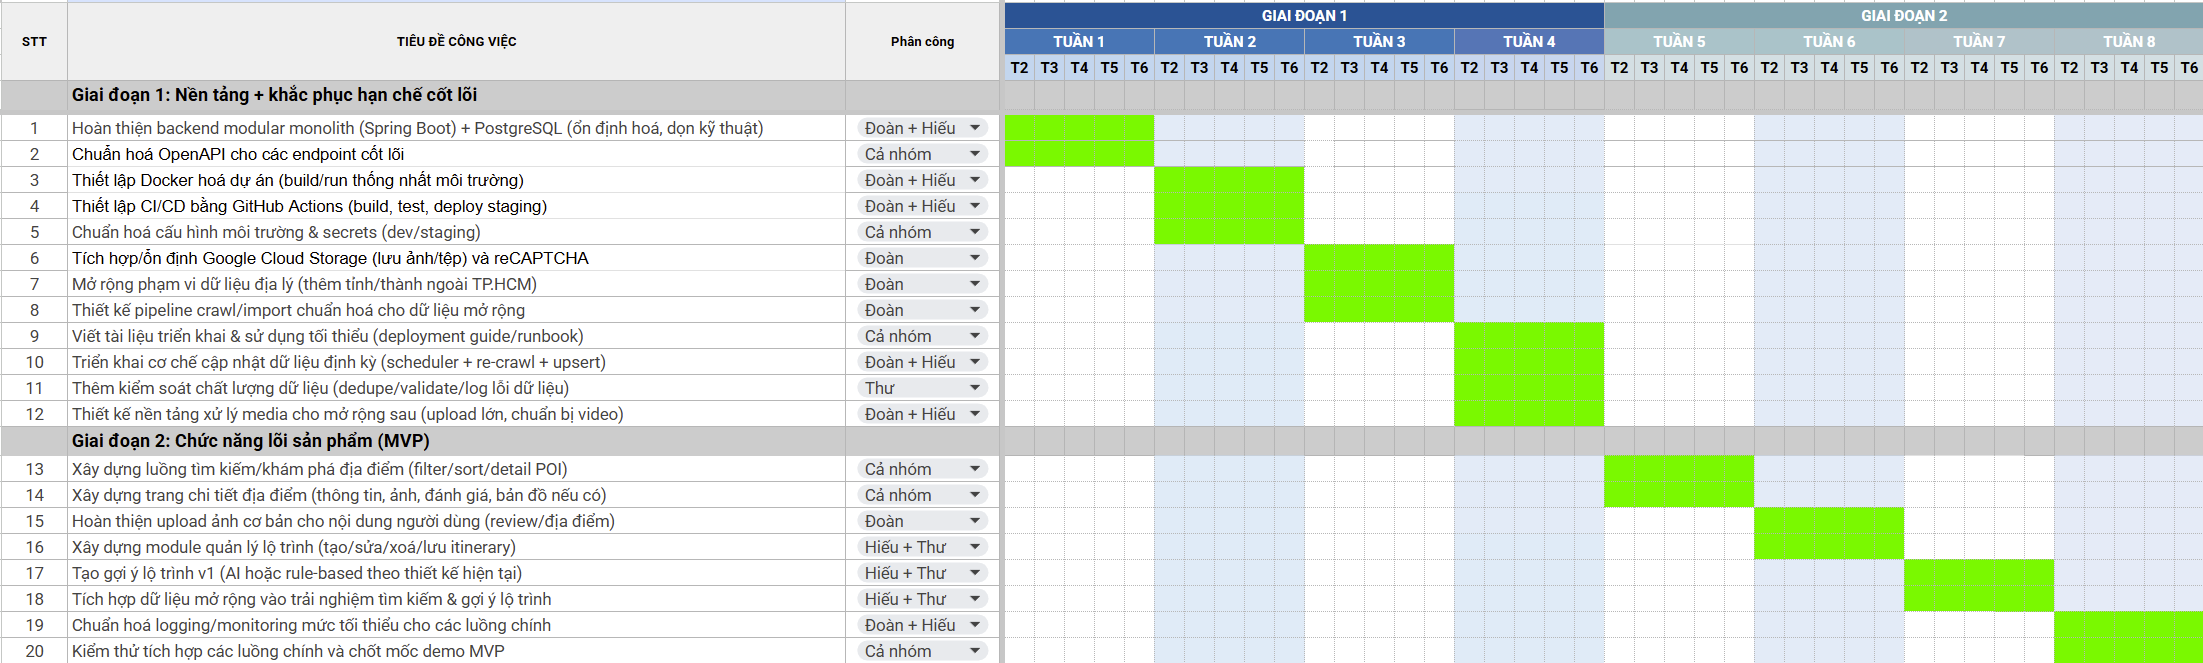
\includegraphics[width=\textwidth]{Images/9. Conclusion/improvement plan first stage.png}
    \caption{Kế hoạch phát triển Giai đoạn 1 và Giai đoạn 2}
    \label{fig:ke-hoach-gd-dau}
\end{figure}

\begin{figure}[htbp]
    \centering
    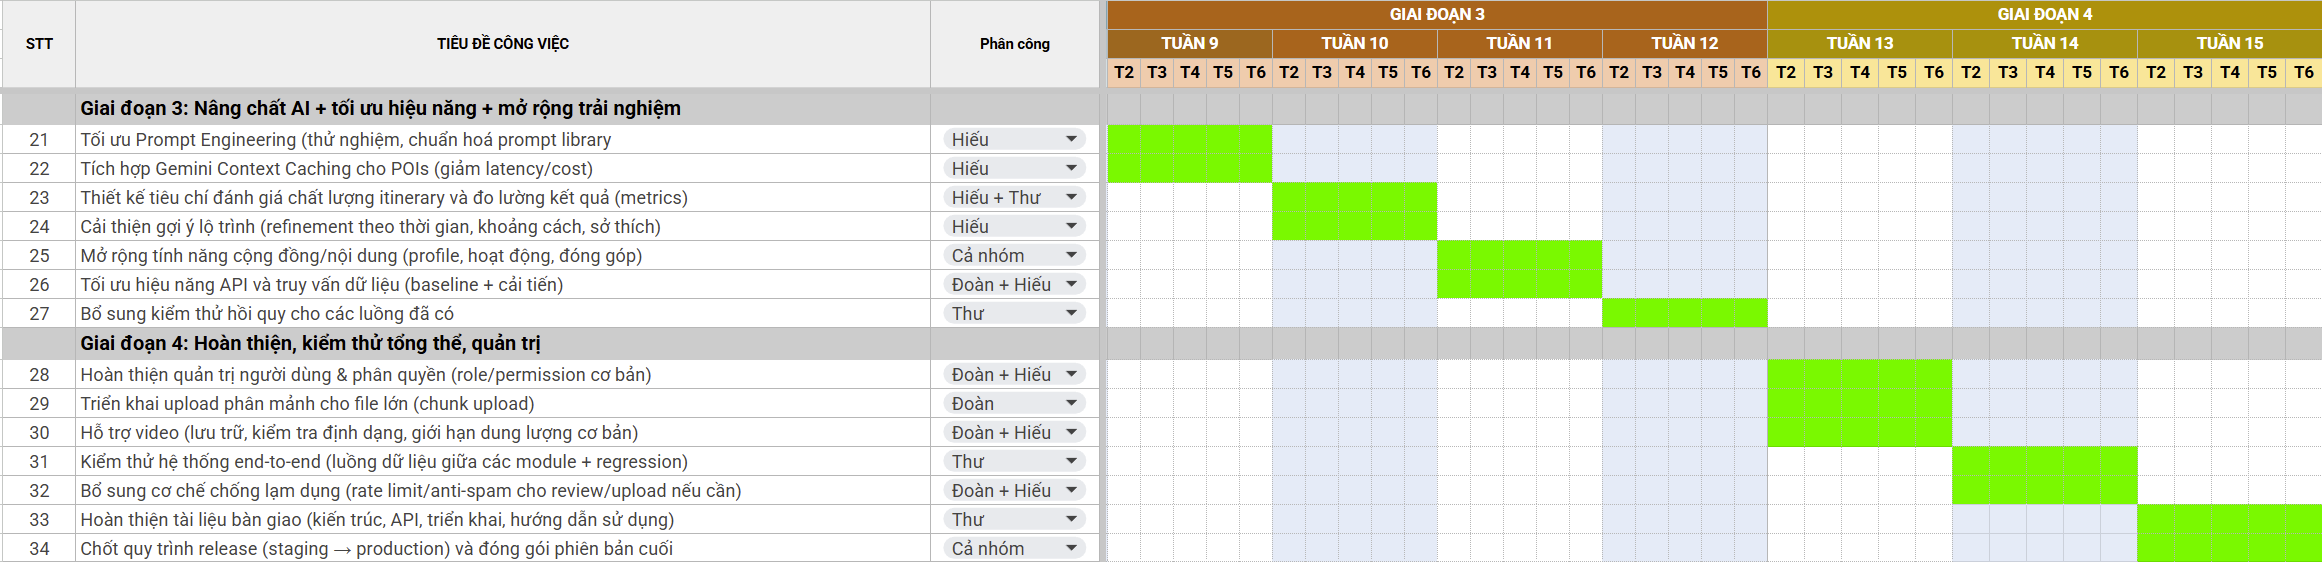
\includegraphics[width=\textwidth]{Images/9. Conclusion/improvement plan second stage.png}
    \caption{Kế hoạch phát triển Giai đoạn 3 và Giai đoạn 4}
    \label{fig:ke-hoach-gd-sau}
\end{figure}

Lộ trình này tập trung vào việc ổn định hệ thống backend trong 4 tuần đầu, xây dựng các chức năng cốt lõi của sản phẩm du lịch như quản lý lộ trình và gợi ý thông minh từ tuần thứ 5 đến tuần thứ 8, và cuối cùng là tối ưu hóa hiệu năng, bảo mật và kiểm thử tổng thể trước khi phát hành phiên bản cuối cùng vào tuần 15.